\documentclass[UTF8]{ctexart}
\usepackage{amsmath}
\usepackage{graphicx}
\usepackage[margin=2.5cm]{geometry}

\title{标题}
\author{author}
\date{date}

\begin{document}

\maketitle
\tableofcontents 
\section{Introduction}

I have learned
\begin{itemize}
	\item title
	\item section
	\item list
\end{itemize}

\section{Result}
this is result section

\subsection{Termial Recorded}
\begin{verbatim}
$ latexmk -pdf -halt-on-error latex_basic.tex
Output written on latex_basic.pdf
Latexmk: All targets are up-to-date
\end{verbatim}

\subsection{Figure}

\begin{figure}
	\centering
	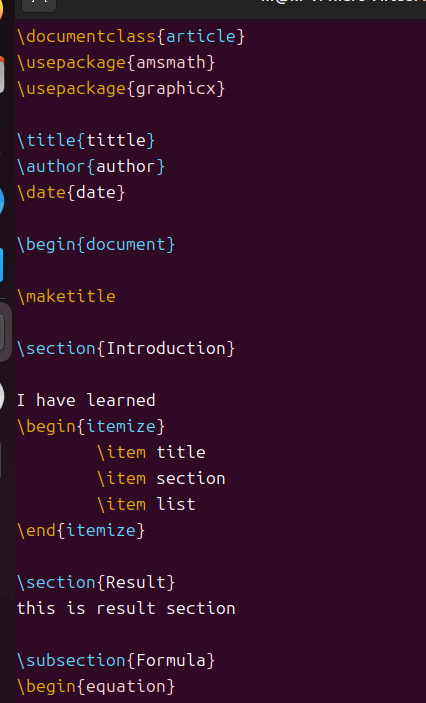
\includegraphics[width = 0.8\linewidth]{image.png}
	\caption{screenshot}
	\label{fig:screenshot}
\end{figure}
Figure~\ref{fig:screenshot} is a screenshot

\subsection{Formula}
\begin{equation}
	T = a + b
	\label{eq:total}
\end{equation}
公式 \ref{eq:total} shows the total

\subsection{Table}
\begin{table}
	\centering
	\caption{toos and result}
	\label{tab:tool-result}
	\begin{tabular}{cc}
		Tools & Result \\
		git & pass \\
		latex & pass \\
	\end{tabular}
\end{table}
this table~\ref{tab:tool-result} show the result and tools

\subsection{Special Character}
I will put my 100\% effort to my career
this is latex\_basic.tex file
shell \& git

\subsection{Build Command}
测试中文支持
this is build command subsection
		\begin{enumerate}
			\item first step writing code
			\item second step compile
			\item third step recompile
		\end{enumerate}

\end{document}
